\documentclass[15pt]{beamer}

\usepackage[utf8]{inputenc}
\usepackage[frenchb]{babel}
\usepackage{beamerthemeSingapore}

% make captions centered
\usepackage[hang, labelfont={sf,bf}, font=footnotesize, margin=2cm]{caption}

% Presentation setup
% list style
\setbeamertemplate{itemize item}[triangle]
\setbeamertemplate{itemize subitem}[triangle]
\setbeamertemplate{itemize subsubitem}[square]

\setbeamertemplate{blocks}[rounded][shadow=true]
\setbeamercolor{block title}{bg=blue!30,fg=black}

\setbeamersize{text margin left = 2em}



\title[Application mobile d'apprentissage]{\textsc{Travaux d’\'Etude et de Recherche} \\Application mobile d'apprentissage}
\author{ \ \ Asmaa \textsc{Sebia}\\
\and Lamia \textsc{M\'eziani}\\
\and Dragos-Adrian \textsc{Seredinschi}}
\institute{Universit\'e d'Orl\'eans, Facult\'e des Sciences\\Département d'Informatique}
\date{May 2012}

\begin{document}

% frame 1 -- title page
\begin{frame}
 \titlepage
\end{frame}


% frame 2
\begin{frame}
 \frametitle{Au sujet du projet}
\begin{itemize}
 \item Sujet: Application mobile d'apprentissage
 \item Particularit\'es:

  \begin{enumerate}
  \setlength{\itemindent}{6em}
  \item[Application mobile] Pour les smartphones, tablettes
  \item[Apprentissage] Trois objectifs: lire, \'ecrire \& compter
  \item[Utilisateurs] Enfants de moins de 5 ans
  \item[Diversit\'e] Prise en charge pour plusieurs langages
  \end{enumerate}

 \item Nom: 
\begin{center}
\textbf{Lire-\'Ecrire-Compter} (LEC)
\end{center}
\end{itemize}
\end{frame}

% frame 3.. about Android
\begin{frame}
 \frametitle{Application mobile pour l'apprentissage}
 \framesubtitle{Syst\`eme d'exploitation - \textbf{Android}}
\begin{enumerate}
 \item<1-> \textbf{Restrictive}, en raison du syst\`eme de fichiers, ressources disponibles, mais..
 \item<2-> \textbf{Avantageux}: écran tactile plus confortable; plus efficace que des sites web,
  plus facile a comprendre et utiliser, notamment pour les enfants
  \begin{center}
  \textsl{Le dispositif mobile augmenter l'apprentissage de manières appropri\'ees} \cite{Marrer2009}
  \end{center}
  \item<3-> \textbf{Dispositifs Android}: beaucoup (plus de 300 millions \cite{AndyR2012}).
  \item<4-> \textbf{Android SDK}: bien document\'e et maintenu; Open Source
\end{enumerate}

\end{frame}

% frame 4.. about learning, in general
\begin{frame}
 \frametitle{Application mobile pour l'apprentissage}
 \framesubtitle{Particularit\'es de l'apprentissage}
\begin{block}{M\'ethodes envisag\'ees}<1->
\begin{enumerate}
  \item Lire
  \item \'Ecrire
  \item Compter
\end{enumerate}
\end{block}

\begin{overlayarea}{\textwidth}{3cm}
\begin{onlyenv}<2>
\begin{exampleblock}{Lire}
Apprendre \`a lire l'alphabet, syllabes, mots, phrases d'une langue.
\end{exampleblock}
\end{onlyenv}

\begin{onlyenv}<3>
\begin{exampleblock}{\'Ecrire}
Apprendre a \'ecrire \`a l'aide de la surface tactile.
\end{exampleblock}
\end{onlyenv}

\begin{onlyenv}<4>
\begin{exampleblock}{Compter}
Apprendre a faire le calcul mental, distinguer les differents chiffres et
operations mathematiques de base.
\end{exampleblock}
\end{onlyenv}
\end{overlayarea}

\end{frame}


% General description of the application
% frame 5
\begin{frame}
 \frametitle{Description g\'en\'erale du logiciel}
 \framesubtitle{Les cas d'utilisation}

Cr\'e\'e en vertu de l'hypoth\`eses que l'utilisateur (enfant):

\begin{enumerate}
 \item<1-> \textbf{Ne peut pas lire} \\
  $\Rightarrow$ beaucoup d'images aussi expressives que possible\\
  $\Rightarrow$ le logiciel doit parler pour atteindre une interactivit\'e
 \item<2-> \textbf{Comprend son langue parl\'ee} \\
  $\Rightarrow$ peut interpreter ce que le logiciel parle
 \item<3-> \textbf{Assist\'ee d'une personne} (au moins au d\'ebut de l'utilisation) - car il 
  pourrait \^etre difficile de naviguer
 \item<4-> \textbf{A le d\'esir d'apprendre et d'exp\'erimenter $\ddot\smile$}
\end{enumerate}
\end{frame}

% frame 6
\begin{frame}
 \frametitle{Description g\'en\'erale du logiciel}
 \framesubtitle{Les cas d'utilisation}
  Ainsi, en dehors de la sp\'ecification du projet, nous avons \'egalement diverses:
  \begin{exampleblock}{Contraintes}<2->
   \begin{itemize}
    \item Navigation facile: \og Keep It Simple \fg{}
    \item Faire parler tout l'information present\'ee
   \end{itemize}
  \end{exampleblock}

  \begin{exampleblock}{Exigences}<3->
   \begin{itemize}
    \item Chaque langage est different, donc pr\^et de parler
    en plusieurs langages.
    \item Differentes niveaux de difficult\'e pour tous les activit\'es
    \item Persister les progr\`es r\'ealis\'es sur une activit\'e
   \end{itemize}
  \end{exampleblock}
\end{frame}

% frame 7 - 
\begin{frame}
 \frametitle{Description g\'en\'erale du logiciel}
 \framesubtitle{Entites du logiciel}
  \begin{itemize}
    \item On peut observ\'e qu'une activit\'e de apprentissage est caract\'eris\'e par plusieurs attributs:
  \begin{enumerate}
   \item Le \textbf{langage} de parler (fran\c cais, anglais, etc..)
   \item La \textbf{m\'ethode} d'apprentissage (lire, \'ecrire, compter)
   \item Le \textbf{niveau} de difficult\'e (plus bas, plus haut, etc..)
   \item L'activit\'e elle-m\^eme - l'\textbf{exercise} qui l'utilisateur est en train a faire
   \item Solutions possibles pour l'exercice courant - \textbf{choix}
  \end{enumerate}
$\Rightarrow$ les entites du logiciel (mod\`ele)
  \end{itemize}
\end{frame}


\begin{frame}
 \frametitle{Description g\'en\'erale du logiciel}
 \framesubtitle{Entites du logiciel - relations}
\begin{itemize}
  \item Une approche hi\'erarchique:
  \begin{center}
    Langage $\stackrel{3}{\longrightarrow}$ M\'ethode $\stackrel{1..*}{\longrightarrow}$ Niveau $\stackrel{1..*}{\longrightarrow}$ Exercise $\stackrel{4}{\longrightarrow}$ Choix
  \end{center}
  \item Remarques:
   \begin{description}
    \setlength{\itemindent}{-2em}
    \item [$\bullet$ 3] M\'ethodes pour chaque langage, parce que nous avons trois objetifs: Lire, \'Ecrire, Compter
    \item [$\bullet$ 4] Choix pour chaque Exercise: l'utilisateur doit choisir une de quatre r\'eponses possibles, seulement une est correcte
    \end{description}
\end{itemize}
\end{frame}


% frame 8 - modular decoupage picture
\begin{frame}
 \frametitle{Architecture du logiciel}
\begin{figure}[tr]
  \centering
  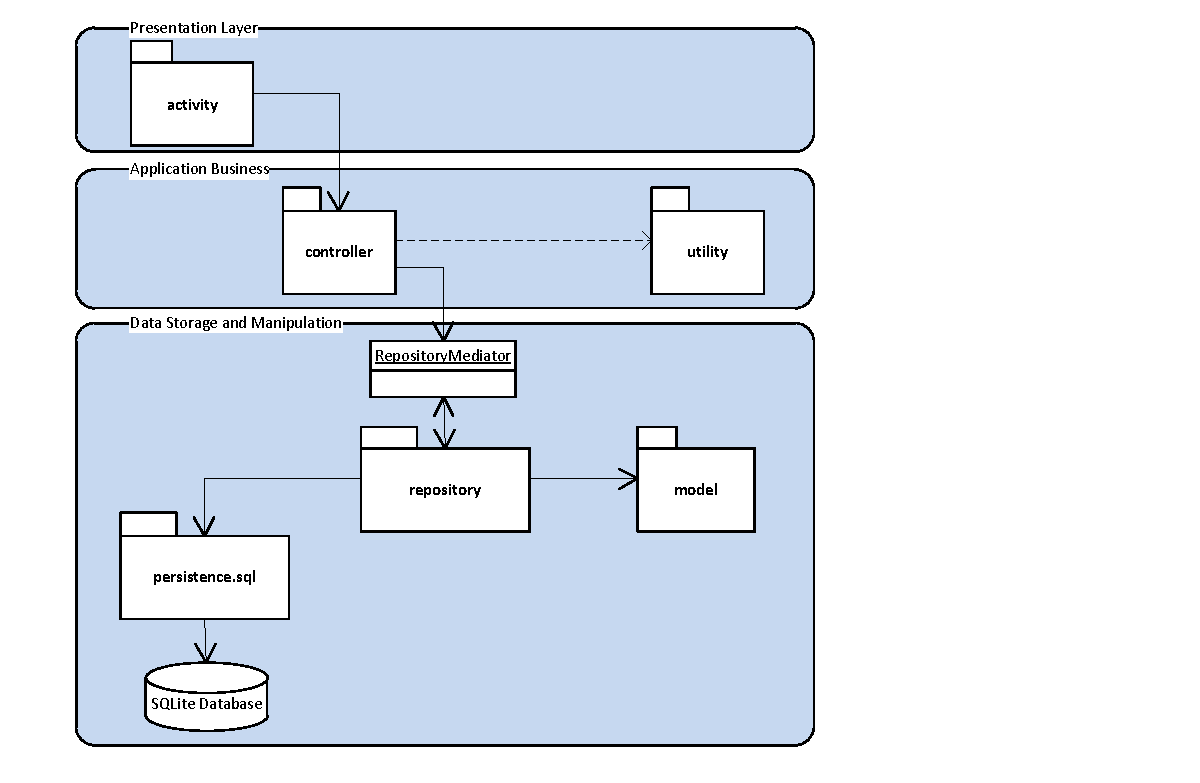
\includegraphics[scale=0.50]{./components.pdf}
  \caption{D\'ecoupage modulaire}
  \label{fig:figure1}
\end{figure}
\end{frame}


% MVC description
\begin{frame}
 \frametitle{Architecture du logiciel}
  \framesubtitle{MVC}
\begin{center}
 M\'ethode de conception: \textbf{Model-View-Controller}
\end{center}

\begin{itemize}
 \item Quelques avantages: 
  \begin{enumerate}
   \item Un plus d'independance entre les composants
   \item Meilleur choix pour notre logiciel qui est centr\'e sur l'utilisateur
   \item Facilite le d\'eveloppement en l'\'equipe
  \end{enumerate}

\item Quelques remarques: 
  \begin{itemize}
   \item View: instances de Android \texttt{Activity} classe
   \item Model: li\'e entre eux par une objet interm\'ediaire - \texttt{RepositoryMediator} - s'assure que les relations sont coh\'erentes et persistantes
  \end{itemize}
 
\end{itemize}
\end{frame}


\begin{frame}
 \frametitle{Architecture du logiciel}
  \framesubtitle{MVC}
\begin{center}
 \item Selon le patron MVC, on peut identifier trois couches pour notre application:
\end{center}

\begin{overlayarea}{\textwidth}{8cm}
  \begin{onlyenv}<2>
    \begin{exampleblock}{View}
      \begin{itemize}
       \item Les activit\'es et les interfaces avec l'utilisateur
       \item \texttt{Activity} classes, et les XML fichiers correspondantes qui d\'ecrit la structure de l'interface
       \item Techniques de parler
       \item Chaque View est li\'e avec un objet Controlleur - pour obtenir les donn\'ees
       \item une \texttt{Activity} sp\'eciale: \texttt{MainActivity} - la classe principale qui d\'emarre l'application
      \end{itemize}
    \end{exampleblock}
  \end{onlyenv}

  \begin{onlyenv}<3>
    \begin{exampleblock}{Controlleur}
      \begin{itemize}
       \item Toutes les affaires du logiciel
       \item Fait le lien entre les donn\'ees et la pr\'esentation
       \item Personnalisation basée sur la langage selection\'e
       \item L'acc\`es aux donn\'ees se fait par le \texttt{RepositoryMediator}
       \item Classe de base abstraite: \texttt{BasicLECController}
      \end{itemize}
    \end{exampleblock}
  \end{onlyenv}

  \begin{onlyenv}<4>
    \begin{exampleblock}{Model (couche de donn\'ees)}
      \begin{itemize}
       \item La plus bas niveau - tout ce qui touche aux donn\'ees
       \item Comprend plusieurs paquets: \texttt{Model}, \texttt{Repository}, \texttt{Persistence}
       \item Fait le lien avec la base de donn\'ees: SQLite\
       \item La base de donn\'ees est initialis\'e lorsque le premier d\'emarrage de l'application,
	  \`a partir d'un fichier XML qui d\'ecrit le contenu et les relations de nos mod\`eles
      \end{itemize}
    \end{exampleblock}
  \end{onlyenv}
\end{overlayarea}
\end{frame}


\begin{frame}
 \frametitle{Points techniques}
  \framesubtitle{Lire}

\begin{itemize}
 \item Le \textbf{synth\`ese vocale} est r\'ealis\'e avec le paquet \texttt{android.speech.tts.TextToSpeech} 
  qui peut \^etre utilis\'e pour plusieurs langages - nous avons
  choisi d'implemented le logiciel avec 3 langages predefinis: \textit{Anglais}, \textit{Fran\c cais}, \textit{Allemand}
 \item Une fois que l'utilisateur a choisit son langage, toute l'interaction est faite dans le langage
  respective
 \item Les exercise de lire sont les plus faciles - l'utilisater doit juste reconna\^itre le lettre / syllabe / mot
  present\'e par l'application
 \item Une \'echelle pr\'esente les progr\`es accomplis jusqu'\`a pr\'esent (\`a l'int\'erieur du m\^eme niveau)
\end{itemize}
\end{frame}


\begin{frame}
 \frametitle{Points techniques}
  \framesubtitle{Compter}

\begin{itemize}
 \item Les exercises de compter ont la m\^eme format que les exercises de lecture, mais l'utilisateur est present\'e
  avec des diverses op\'erations math\'ematiques simples
 \item Nous avons identifi\'e des probl\`emes avec \texttt{android.speech.tts.TextToSpeech}, pour les op\'erations de
  diff\'erence (e.g. $4-1=3$), l'operator \og$-$\fg{} n'est pas prononc\'e correctement
\end{itemize}
\end{frame}


\begin{frame}
 \frametitle{Points techniques}
  \framesubtitle{\'Ecrire}

\begin{alertblock}{\'Ecriture}
\begin{itemize}
\item Normalement, les activit\'es d'\'ecriture se composer de plusieurs exercises dans lequel l'enfant
  essayer de faire les symboles donn\'ees comme exemple \\
$\Rightarrow$ dans une tablette, l'enfant doit essayer de la m\^eme mani\`ere et le logiciel doit \textbf{reconna\^itre}
si l'\'ecriture est correct ou pas
\end{itemize}
\begin{center}
 {\color{red} \textbf{Pas facile!}}
\end{center}
\end{alertblock}

\begin{itemize}
\item Les autres points techniques sont semblable avec les ceux des l'autres types d'activit\'es
\end{itemize}
\end{frame}


% Exemples 
\begin{frame}
 \frametitle{Exemples de fonctionnement}
  \framesubtitle{Page d'accueil}
\begin{figure}[tr]
  \centering
  
\includegraphics[scale=0.50]{./home.png}
  \caption{La premi\`ere page contient 3 drapeaux et chaque drapeau représente une langue d'apprentissage.}
  \label{fig:figure1}
\end{figure}
\end{frame}

\begin{frame}
 \frametitle{Exemples de fonctionnement}
  \framesubtitle{Presentation des m\'ethodes}
\begin{figure}[tr]
  \centering
  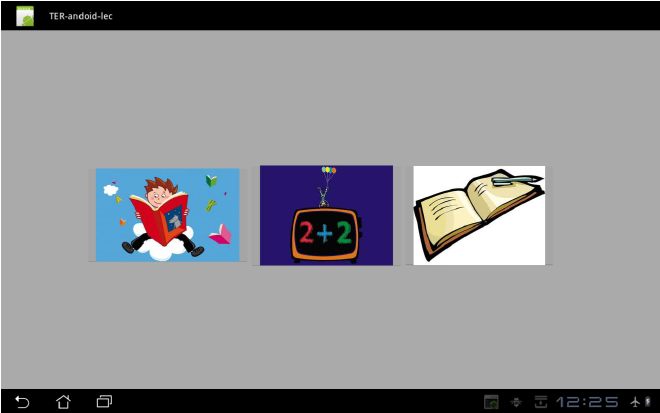
\includegraphics[scale=0.50]{./methods.png}
  \caption{La deuxi\`eme page contient les 3 m\'ethodes disponibles.}
  \label{fig:figure1}
\end{figure}
\end{frame}

\begin{frame}
 \frametitle{Exemples de fonctionnement}
  \framesubtitle{Les niveaux}
\begin{figure}[tr]
  \centering
  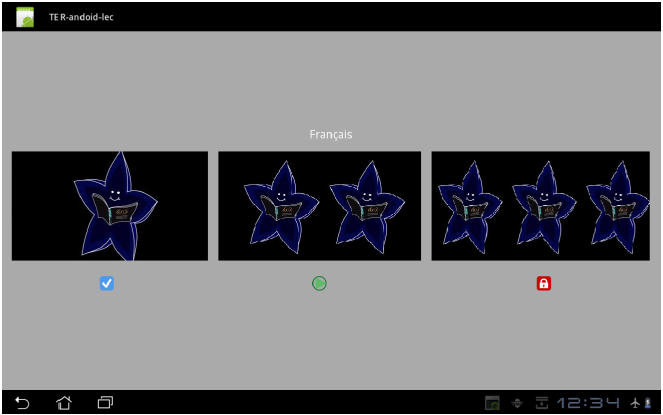
\includegraphics[scale=0.50]{./levels.png}
  \caption{Apres une m\'ethode est choisit, les niveaux sont present\'ees. Ici, l'utilisateur a complet\'e le pr\`emiere niveau.}
  \label{fig:figure1}
\end{figure}
\end{frame}

\begin{frame}
 \frametitle{Exemples de fonctionnement}
  \framesubtitle{Une exercise}
\begin{figure}[tr]
  \centering
  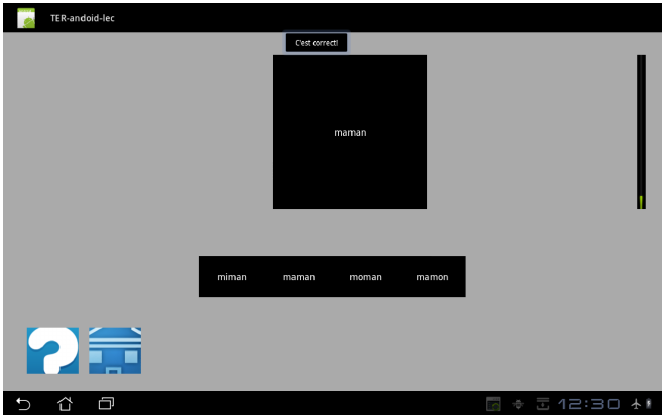
\includegraphics[scale=0.50]{./exercise.png}
  \caption{Exemple de fonctionnement d'une exercise de type \textit{Lire}, pour le langage \textit{Fran\c cais}.}
  \label{fig:figure1}
\end{figure}
\end{frame}


\begin{frame}
 \frametitle{Extensions possibles}
\begin{enumerate}
 \item Le logiciel est facile a \'etendre - pour ajouter des autres langages:
  \begin{enumerate}
    \item Modifier juste le fichier XML qui d\'ecrit la base de donn\'ees
    \item faire de la place (avec le drapeau) dans la page d'accueil
  \end{enumerate}
 \item Le m\'ethode d'\'ecrire!
 \item Multi-utilisateurs: Cr\'eation des comptes pour les enfants et les instituteurs
  \begin{enumerate}
    \item Modifier le fichier XML qui d\'ecrit la base de donn\'ees
    \item Ajouter les classes de mod\'eles, view \& controlleur necessaires
  \end{enumerate}
 \item Personnaliser l'\'echelle: plus convivial - suffit de modifier le 
  widget qui d\'ecrit l'\'echelle
\end{enumerate}
\end{frame}


% Bibliography.. important

\begin{frame}
\frametitle{Bibliographie}

\begin{thebibliography}{10}
  \bibitem[Marrer G., 2009]{Marrer2009}
  Marrer G.
  \newblock A Mobile Learning Definition for My Campus, 2009.

  \bibitem[Andy Rubin, 2012]{AndyR2012}
  Andy Rubin
  \newblock Android@Mobile World Congress: It’s all about the ecosystem, 2012.

\end{thebibliography}

\end{frame}

 %[Marrer G., 2009] Marrer G. A Mobile Learning Defnition for My Campus,2009

\end{document}
